\setlength{\footskip}{8mm}

\chapter{INTRODUCTION}

\section{Background of the Study}

Previous outbreaks of \ac{s.agalac}\label{acro:s.agalac} and \ac{a.veronii} in \aca{onilo}, Oreochromis niloticus, were reported in Japan, Taiwan, and the United States. \ac{a.veronii} and \ac{s.agalac} are widespread pathogens of \aca{onilo} world-wide  and induce mass mortality of the fish in a few days. The two bacterial isolates used in this research are from Thailand, where the bacteria are present and create substantial economic losses for Thai aquaculture industry.

\section{Statement of the Problem}

In order to sustain an intensified and resilient Cichlids' aquaculture, many research units and private companies around the world are studying immune responses of fish to viral and bacterial infections and are experimenting with vaccines development. There is currently no existing vaccine against the \ac{s.agalac} and \ac{a.veronii}. Oil-based \ac{fkv} can be used as a prophylaxis treatment for aqua-cultured freshwater fish and this method is cost efficient and a viable alternative for the \aca{onilo} that has not yet been developed in Thailand. A combined vaccination with a bivalent vaccine is the most cost-effective solution.

\section{Hypothesis}

Previous literature has shown the possibility to develop monovalent and multivalent vaccines for fish such as Asian seabass using whole inactivated pathogens. Assumption that Asian seabass and \aca{onilo} share a similar physiology and similar dynamics in their response to \ac{ag} support the possibility of making a vaccine for the \aca{onilo}.

My second assumption is the feasibility of the \acs{fkv} vaccine production using low-cost method with pathogen inactivation using a chemical: formalin with concentration of 1\% - 3 \acs{(v/v)}, which would make the vaccines cost-efficient for farmers and medium sized farms. 

\section{Objectives of the research project} 

The objective of this research is to create new cost-effective vaccines in the Nile Tilapia against two fish pathogens \ac{s.agalac} and \ac{a.veronii}.

The three vaccines developed are in the table 1:

\addcontentsline{lot}{chapter}{Table 1 \hskip 3.55em Summary of the inactivated vaccines used in the study }
\begin{center} 
  \caption{\textbf{Table 1}
  \textwidth
  \begin{tabular}{ll}
    \ac{a.veronii} & \ac{av} \\
    \ac{s.agalac} & \ac{sa} \\
    \ac{s.agalac} + \ac{a.veronii} & \ac{saav} 
  \end{tabular}
\end{center}

The vaccines will be \aca{ip} (\ac{ip}) in order to understand the elicited systemic and mucosal immune response of \aca{onilo}. In addition, the efficiency of the monovalent formulations (\ac{sa},\ac{av}) is compared versus the bivalent formulation (\ac{saav}) will be compared with a challenge test.

\section{Risks and limitations}

\subsection{Access to laboratory facilities}

The experiments will be held and conducted at Asian Institute of Technology in the AARM department (stocking of fish and vaccination and challenge) and at SSRU laboratory facilities (\ac{elisa}, agglutination test, \ac{rtpcr}) and eventually at Mahidol Centex Shrimp.

\subsection{Safety of experiments}

Culture of the bacteria might not cause a risk to the wild fish and environment because all the experimentations will be made in closed and hermetic culture systems with compliance and respect of the strict biosecurity rules. 

\subsection{Risks in the schedule}

The main challenges and risks could be due to any delays related fish keeping and fish culture or due to problems in the bacterial culture or vaccine preparation. It could eventually lead to a delay in the realization of the research project.

\section{Organization of the research project}

\subsection{Project fundings}

The project funding will come from the support of the AIT Innovative research fund.

\subsection{Organization of the research project}

I have divided my work in work packages.

I organize the rest of this research thesis as follows.

I have broken down the project work in several phases as shown in Figure 1.

In Chapter \ref{ch:literature-review}, I describe the literature review.

In Chapter \ref{ch:methodology}, I propose my methodology for the experimental design, for the pond preparation, the fish feeding regime. But also for bacterial culture, vaccination, fish mucus swabs and blood sampling. For antibody agglutination titration, \ac{elisa}, \ac{rtpcr} and finally for the Challenge tests. 

In Chapter \ref{ch:results}, I present the experimental results.

Finally, in Chapter \ref{ch:conclusion}, I conclude my thesis.

\beginfigure
  \begin{center}
  \begin{flushleft}
  \caption{\textbf{Figure 1: Steps of the research project}} \\
  \end{flushleft}\\
  \\
  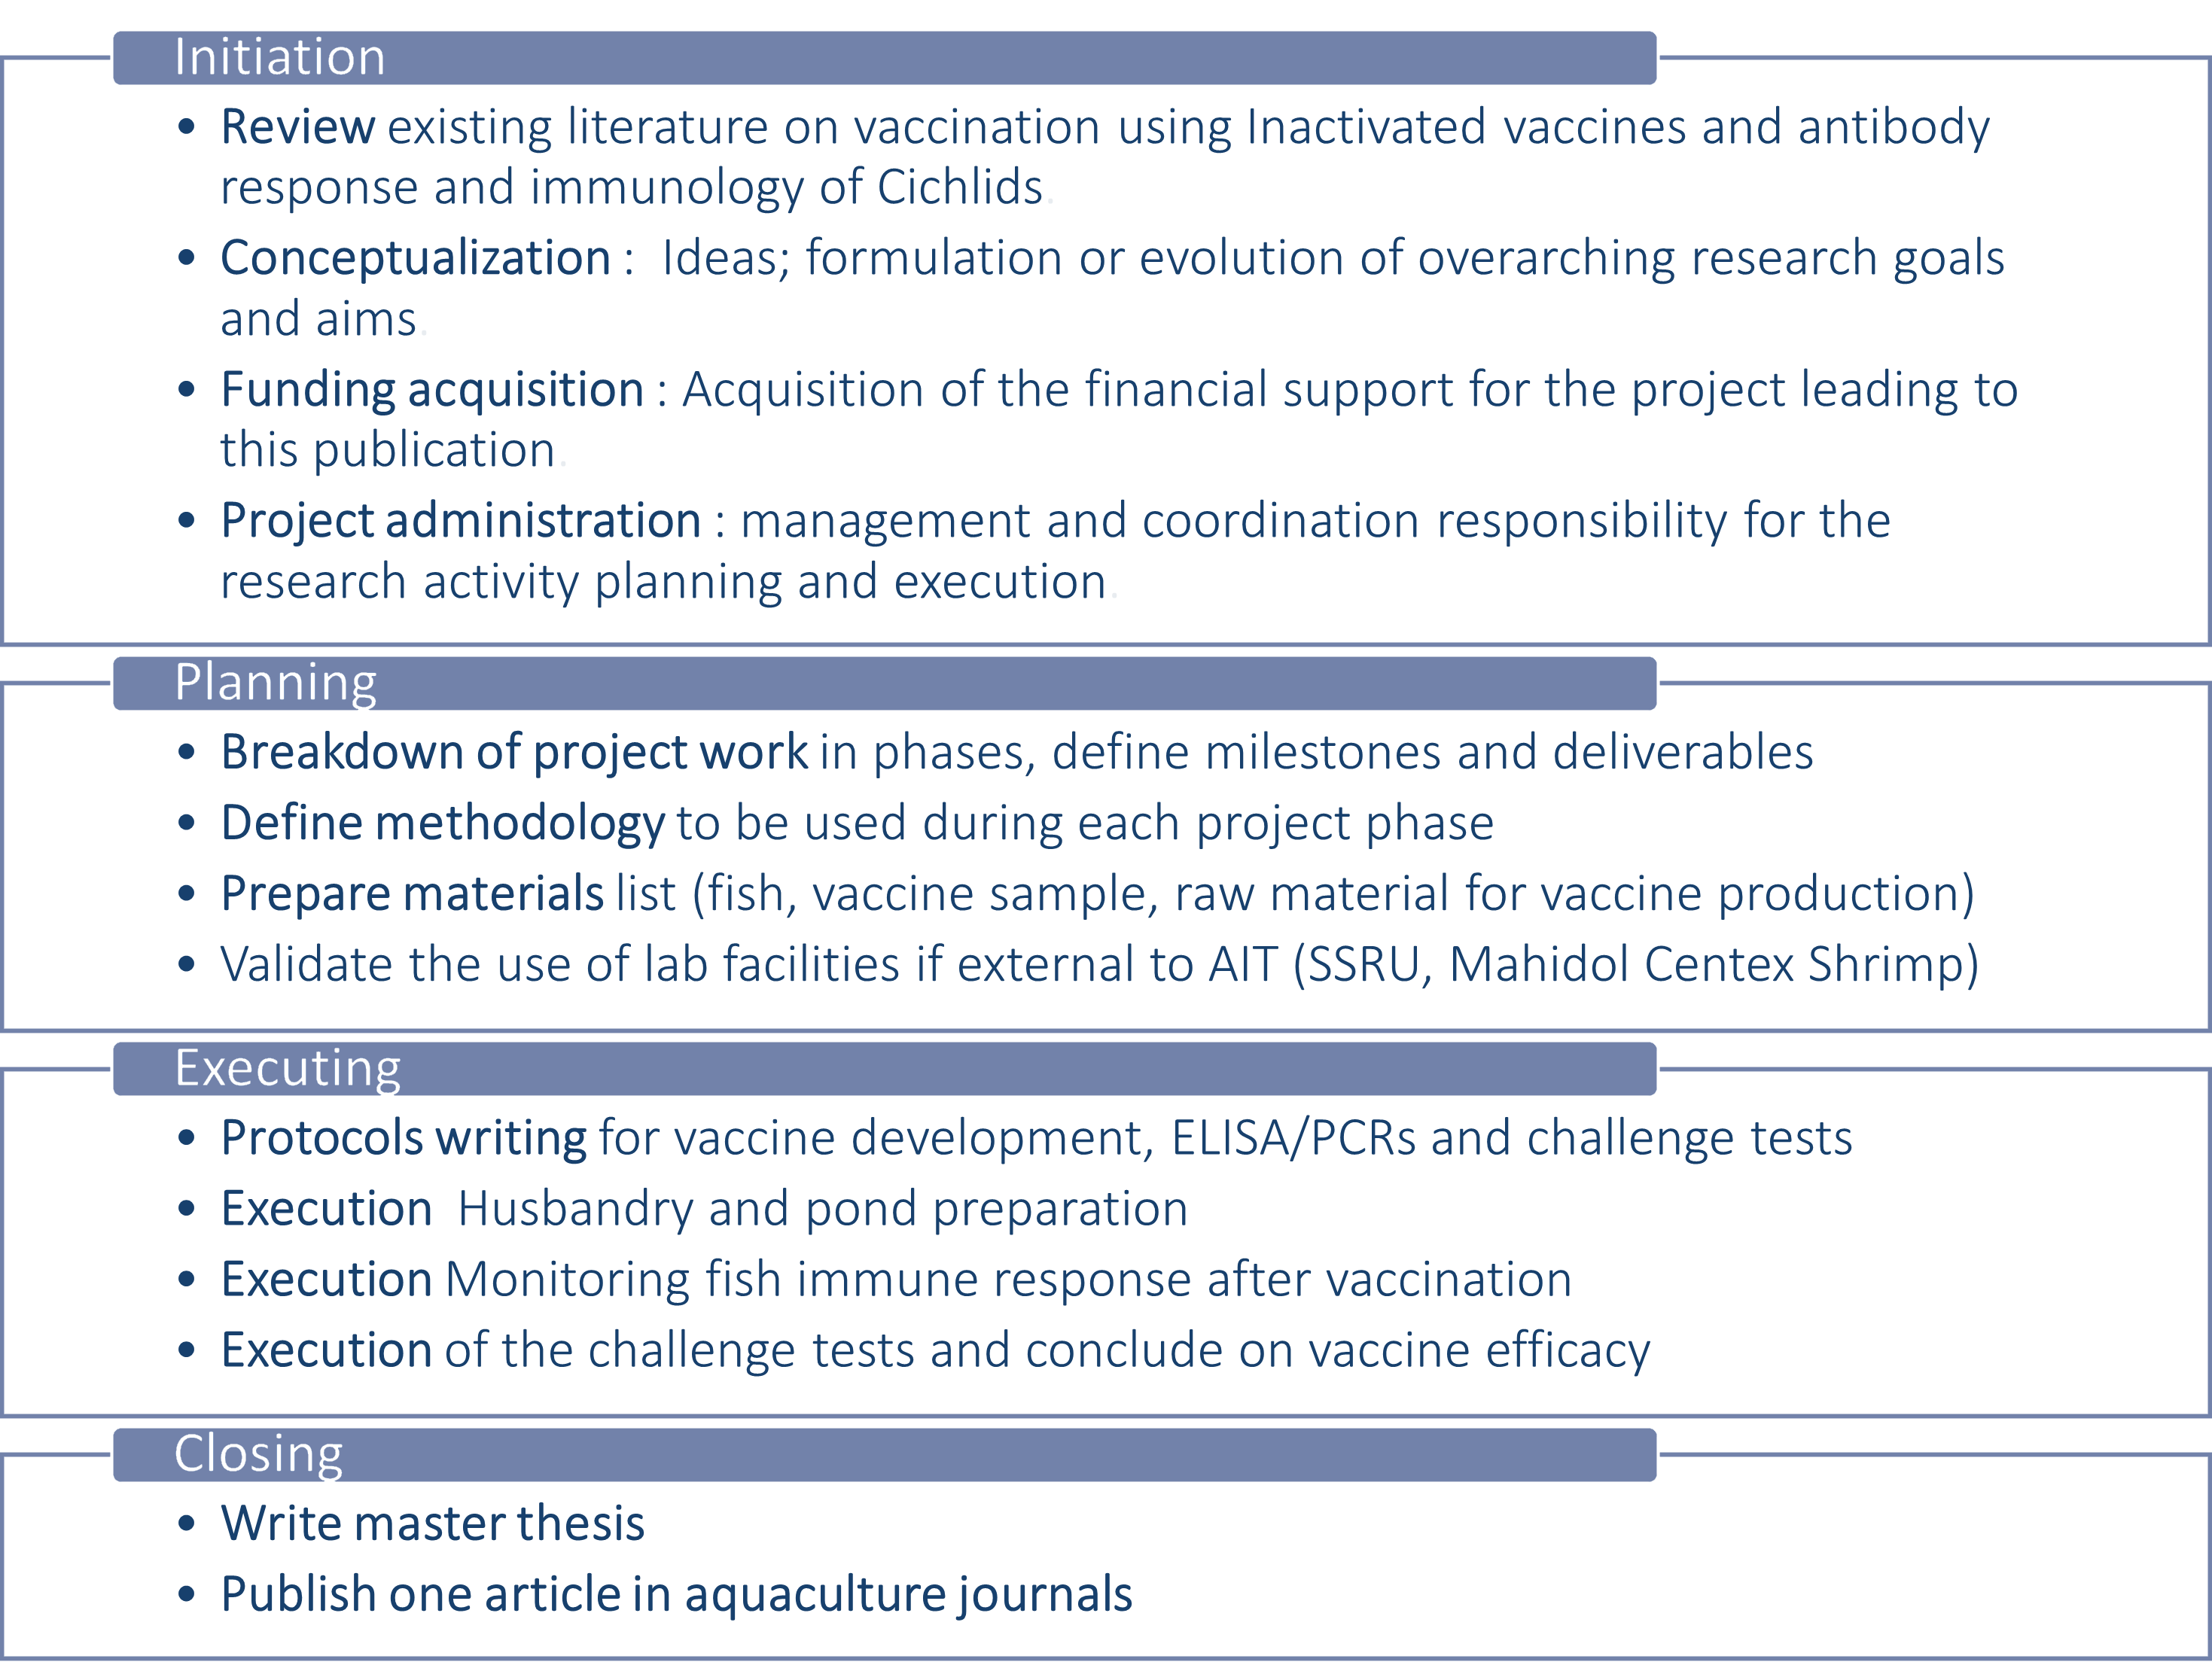
\includegraphics[width=\textwidth, height=\textheight, 
                 keepaspectratio]{figures/Figure1.png}
  \label{figure 1: The research plan}
  \addcontentsline{lof}{chapter}{Figure 1 \hskip 3.55em Organization of the research project}
  \endfigure
  \end{center}
\FloatBarrier
